\section{Clustering}
At the beginnig of our research we tried to find a pattern that could relate the style of the player ( \textit{rel ace},  \textit{rel df},  \textit{rel 1stIn},  \textit{rel 1stWon},  \textit{rel 2ndWon}) with respect to his strength.\\ After feature engineering, clustering and analysis we found no meaningful results. So, we decide to switch to the analysis that we will present in this report.

\subsubsection{Features selection}
We have decided to select the features respecting the following criteria in order
\begin{itemize}
    \item Selection of those features that may provide an interesting picture about the performance of the players.
    \item Dropped all the couple of features that have more than `70\%` of correlation. Leaving just one feature per correlated pair.
    \item Removed features deemed unimportant that had a good percentage of null values.
\end{itemize}

% Since in the player's dataframe there was a big number of records with NaN values, corresponding to the in-match statistics (rel\_ace, rel\_df, rel\_1stIn etc.), we set a threshold establishing that every player in order to be in the dataframe should have played at list 15 matches with non-null values for these features.
% Then we selected the features which seemed to better represent the “strength” of a player, and we performed the correlation analysis (Fig. \ref{fig:correlation_plot}) in order to have a narrower selection. Whenever two features had a correlation greater than 70\% (Pearson coefficient), we discarded one of the two. 
As a results we obtained the following uncorrelated features:
\begin{center}
    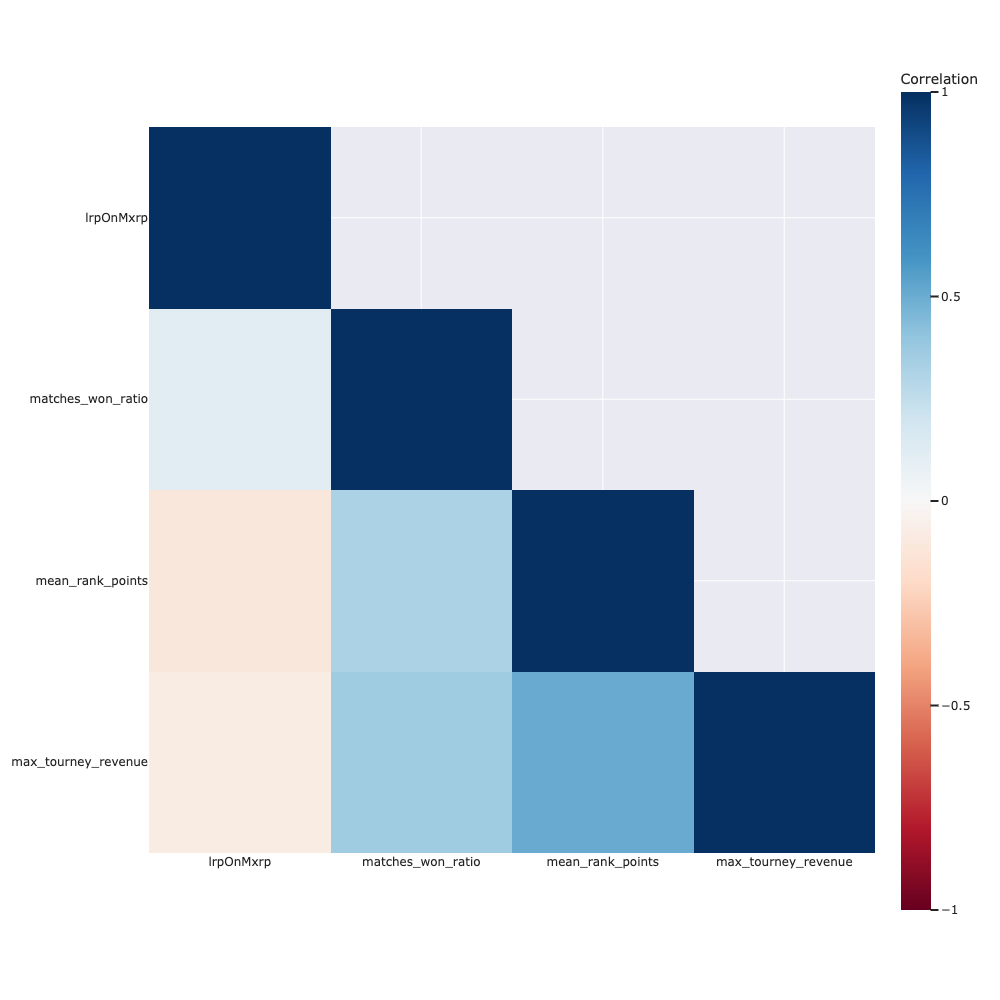
\includegraphics[width=350px]{plots/correlation_plot}
    \label{fig:correlation_plot}
    \captionof{figure}{Correlation Plot}\label{fig1}
\end{center}
At this point the remaining features were: 'lrpOnMxrp', '\textit{matches\_won\_ratio}', '\textit{mean\_rank\_points}',\\ '\textit{mean\_tourney\_spectators}', '\textit{max\_tourney\_revenue}'.\\
Those features will be used as a starting point in the clustering.

\subsubsection{Additional Cleaning}
Before clustering, we had to perform additional cleaning to ensure:
\begin{itemize}
    \item There were no null values present in the data: by dropping nan values from \textit{lrpOnMxrp} feature.
    \item Higher quality data: after iterating between feature selection and clustering, we found out that by filtering players just by taking the one who played at least 15 games, we were able to gain higher quality results.
\end{itemize}
\subsection{K-means}

\subsubsection{Distributions and preprocessing}
Being K-means suitable for globular cluster, we decided to perform logarithm to the \textit{mean\_rank\_points} feature that follow a power law to lead to a more compact distribution:
\ref{fig:mean_rank_points}  \ref{fig:log_mean_rank_points}.

\begin{figure}[h]
\centering
\begin{minipage}{.5\textwidth}
\centering
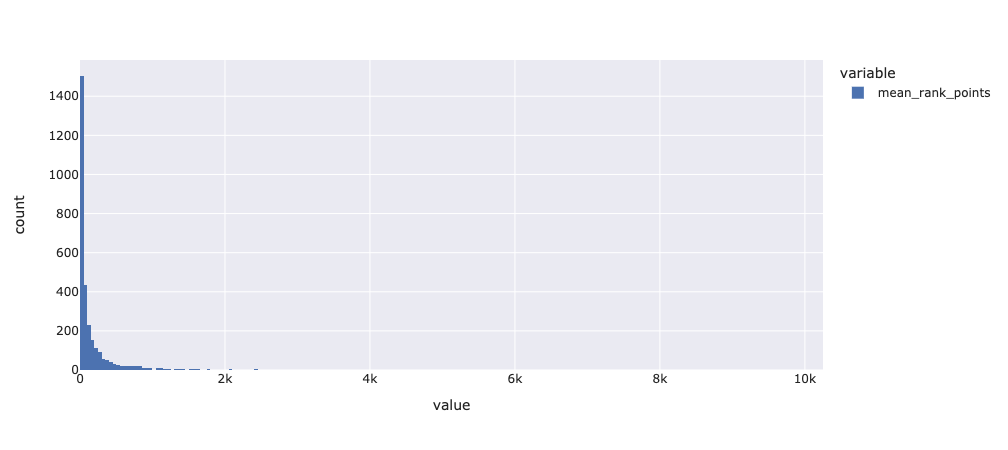
\includegraphics[width=\textwidth]{plots/kmeans/preprocessing/mean_rank_points}
\captionof{figure}{Mean rank points}
\label{fig:mean_rank_points}
\end{minipage}%
\begin{minipage}{.5\textwidth}
\centering
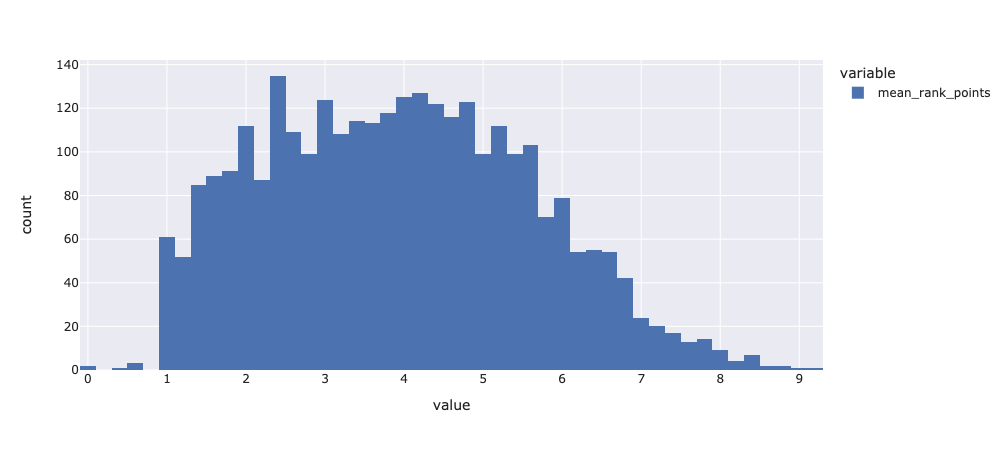
\includegraphics[width=\textwidth]{plots/kmeans/preprocessing/log_mean_rank_points.png}
\captionof{figure}{Variance rank points}
\label{fig:log_mean_rank_points}
\end{minipage}
\end{figure}

\subsubsection{Optimal K}
The optimal choice for k was done by following the elbow rule, that suggested to use $k=4$ where the SSE score was 185.316 (Fig. \ref{fig:kmeans_elbow_rule}). The clusters were fairly balanced and all of them crossed the Average Silhoutte Score of 0.47 (Fig. \ref{fig:kmeans_silhouette_score}). In other words, the closer it is to one, the better the object is matched to its own cluster and poorly matched to neighbouring clusters.


\begin{figure}[!h]
\centering
\begin{minipage}{.5\textwidth}
\centering
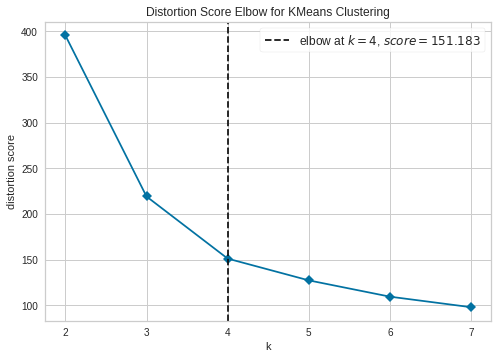
\includegraphics[width=\textwidth]{plots/kmeans/kmeans_elbow_rule}
\captionof{figure}{Elbow rule}
\label{fig:kmeans_elbow_rule}
\end{minipage}%
\begin{minipage}{.5\textwidth}
\centering
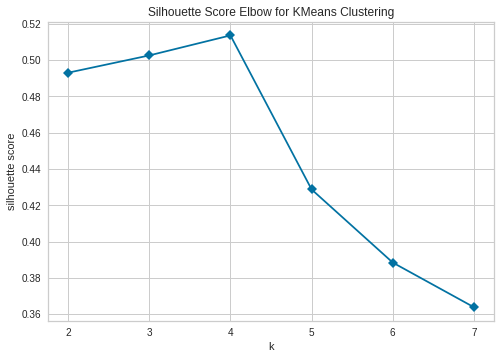
\includegraphics[width=\textwidth]{plots/kmeans/kmeans_silhouette_score}
\captionof{figure}{Silhouette score}
\label{fig:kmeans_silhouette_score}
\end{minipage}
\end{figure}

\subsubsection{Results interpretation}
Clustering does not clearly distinguish between classes of players, however it is possible to find fairly defined patterns by observing the following histograms (\ref{fig:total_match_played_kmeans}, \ref{fig:mean_rank_points_kmeans}, \ref{fig:age_kmeans}, \ref{fig:lrpOnAvgrp_kmeans}) and the plot related to the centroids  and the plot regarding the centroids (\ref{fig:kmeans_results}).

% \begin{itemize}
%     \item{ \textbf{Cluster 0} represents the young promises: those with low mean\_rank\_points, an average low age and on average the ones with the strongest trends of growth (looking at the \textit{lrpOnAvgrp}).}
%     \item{ \textbf{Cluster 1} represent the strongest players: with experience and a generally higher age. They have high mean\_rank\_points and perform the best in term of matches won ratio.}
%     \item{ \textbf{Cluster 2} represent good players with a decreasing trend.}
%     \item{ \textbf{Cluster 3}: represents the bad players: with low mean\_rank\_points and a decreasing trend.}

% \end{itemize}

\begin{figure}
\centering
\begin{minipage}{.5\textwidth}
\centering
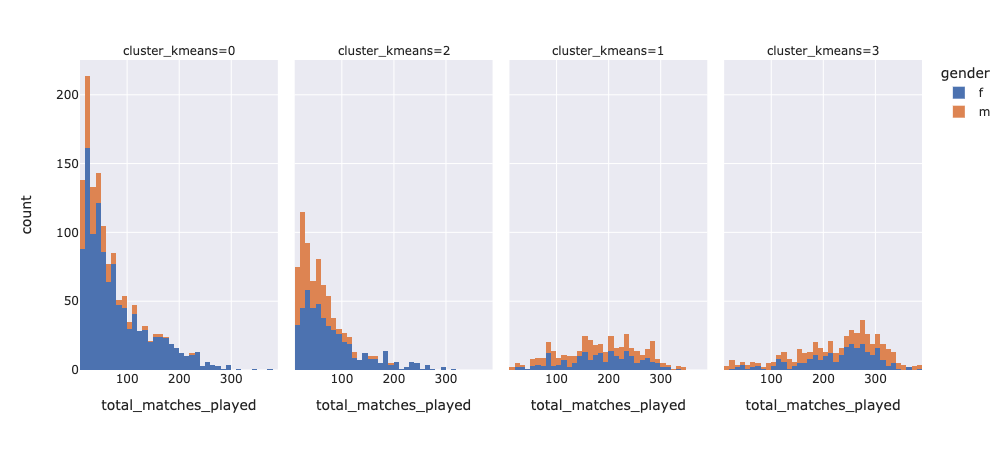
\includegraphics[width=\textwidth]{plots/kmeans/hist_total_matches.png}
\captionof{figure}{total\_matches\_played histogram}
\label{fig:total_match_played_kmeans}
\end{minipage}%
\begin{minipage}{.5\textwidth}
\centering
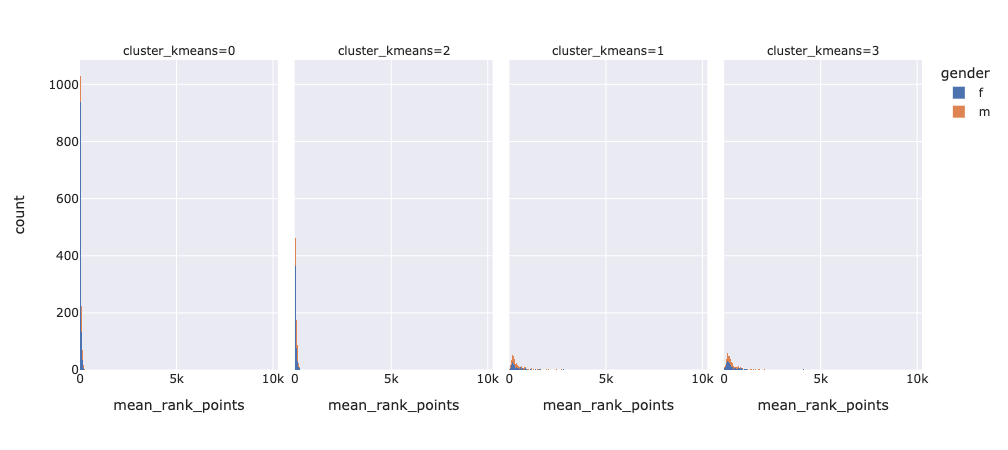
\includegraphics[width=\textwidth]{plots/kmeans/hist_mean_rank_points.png}
\captionof{figure}{mean\_rank\_points histogram}
\label{fig:mean_rank_points_kmeans}
\end{minipage}

\centering
\begin{minipage}{.5\textwidth}
\centering
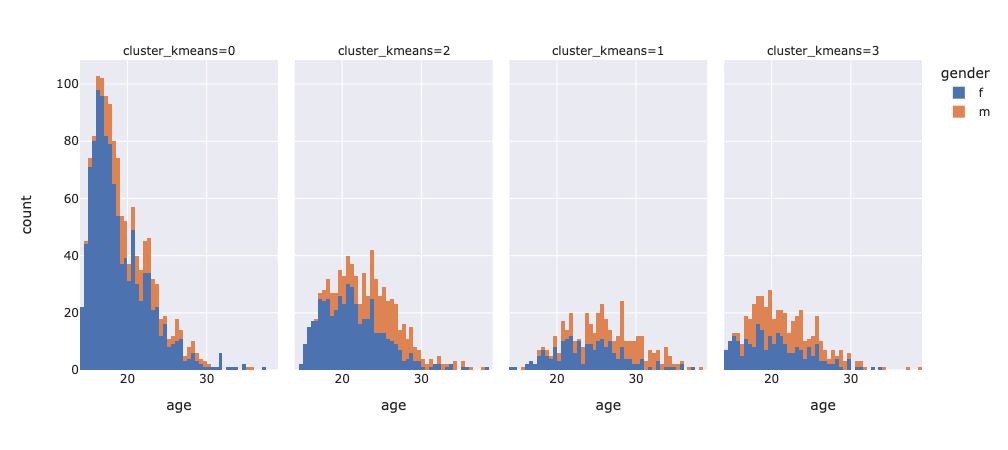
\includegraphics[width=\textwidth]{plots/kmeans/hist_age.png}
\captionof{figure}{age histogram}
\label{fig:age_kmeans}
\end{minipage}%
\begin{minipage}{.5\textwidth}
\centering
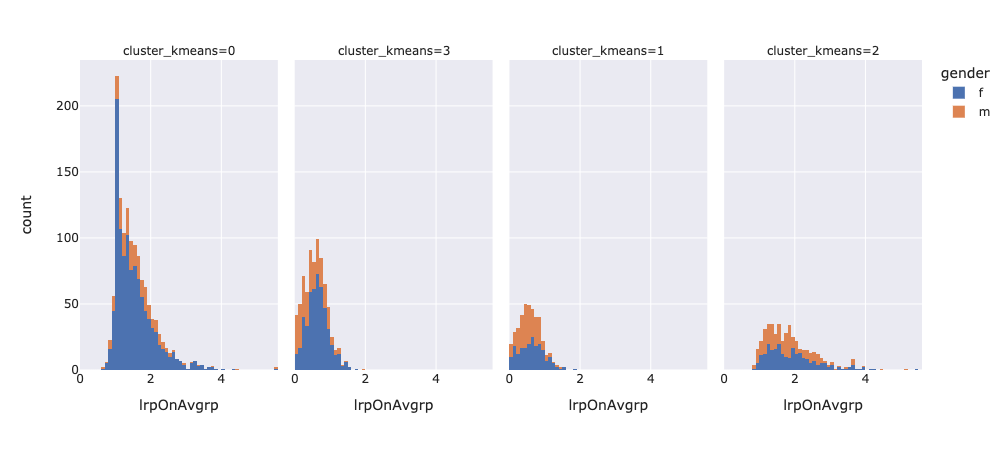
\includegraphics[width=\textwidth]{plots/kmeans/hist_lrpOnAvgrp.png}
\captionof{figure}{lrpOnAvgrp histogram}
\label{fig:lrpOnAvgrp_kmeans}
\end{minipage}
\end{figure}

\begin{figure}[h]
\centering
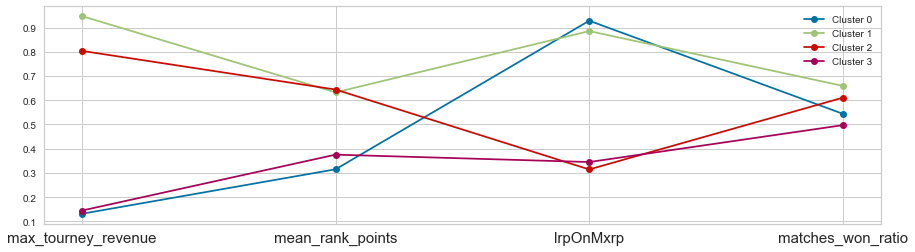
\includegraphics[width=\textwidth]{plots/kmeans/kmeans_results}
\captionof{figure}{Results of K-means}
\label{fig:kmeans_results}
\end{figure}



\newpage

\subsection{Density based}
The set of feature used for DBSCAN is the same as Kmeans as well as for the applied transformations.\\
To understand a good range of values for eps we print the following plot \ref{fig:dbscan_distances} to check the distances between the k-th nearest values for each possible point. Each distance is plotted in the x axis ordered with respect to the k-th nearest value.

\begin{figure}[h]
\centering
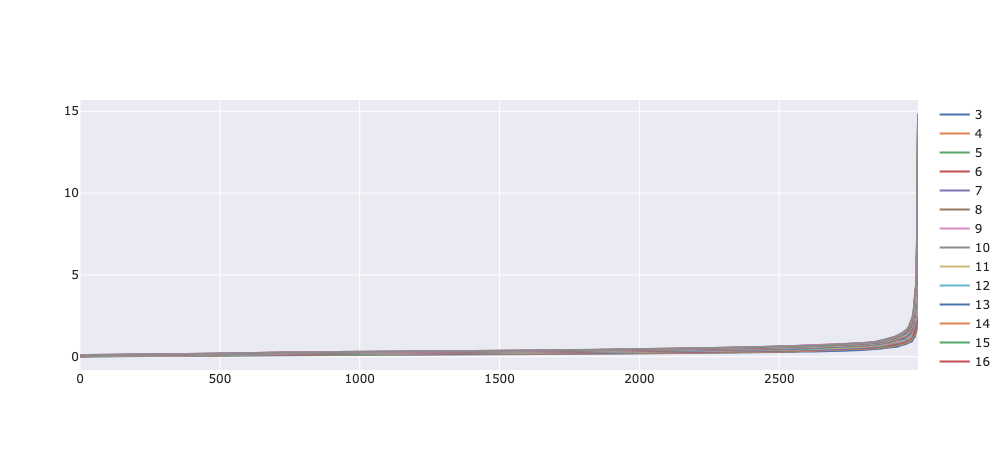
\includegraphics[width=\textwidth]{plots/dbscan/dbscan_distances}
\captionof{figure}{Noise points with the k-th nearest neighbor at farther distance}
\label{fig:dbscan_distances}
\end{figure}

Then we run a grid-search using as a range of values for eps = $[0.1, 2.9]$ \ref{fig:dbscan_metrics}. Through the grid search in combination with the k-th distance plot (\ref{fig:dbscan_distances}) , we could get a better understanding of the kind of results we could expect for each rank and the resulting number of clusters.

\begin{figure}[h]
\centering
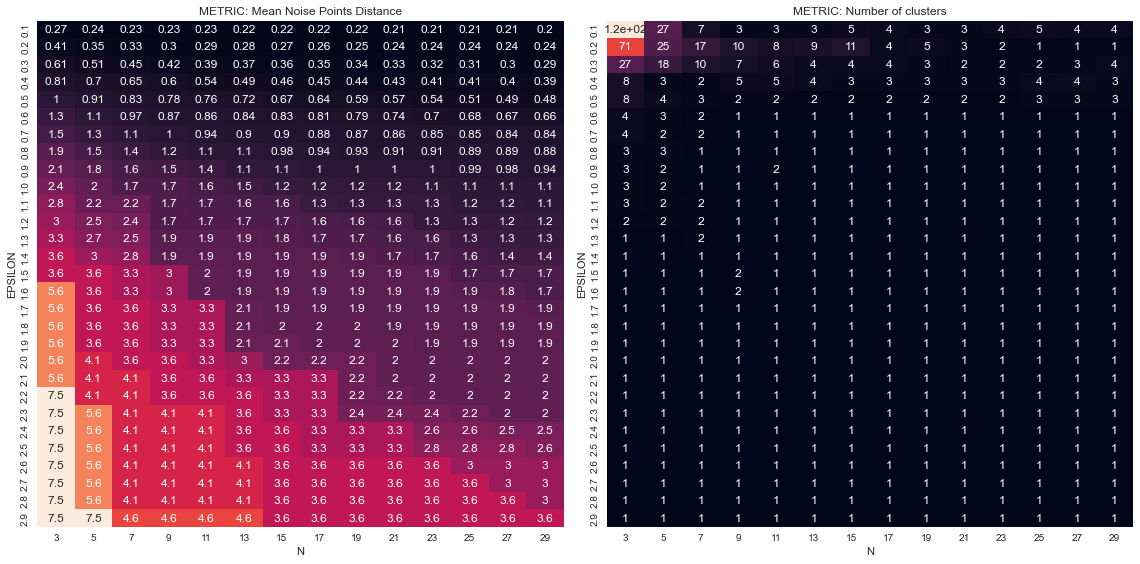
\includegraphics[width=.6\textwidth]{plots/dbscan/dbscan_metrics}
\captionof{figure}{Chosen hyper-parameters $eps=1$ and $n=3$}
\label{fig:dbscan_metrics}
\end{figure}

\subsubsection{Results interpretation}
With most combinations of hyperparameters the clusters results unbalanced and there were an high number of outliers.
However assigning $eps=1$ and $n=3$ (AGGIORNARE GLI IPERPARAM) the results are satisfactory.

The clusters result fairly balanced in the number of elements, except from a smaller cluster composed of just three top players: Roger Federer, Simona Williams and Simona Halep
The noise labelled by DBSCAN was none other than very bad o very good player.
The two remaining clusters represented either good or bad players in term of \textit{mean\_rank\_points} or \textit{matches\_won\_ratio}.

\begin{itemize}
\item \textbf{Cluster 1 , 2, -1}
    \begin{itemize}
        \item The promises (Cluster 1): Pretty strong ranking with extreme growth and very young.
	    \item Cluster 2: Strong players and pretty young
	    \item The veterans (Cluster -1), DBscan classified the outliers as the strongest players. The strongest, the oldest and with a growing score.
	 \end{itemize}
\item \textbf{Cluster 0}: The bigger cluster, relative to the remaining larger group
\end{itemize}	

\begin{figure}[h]
\centering
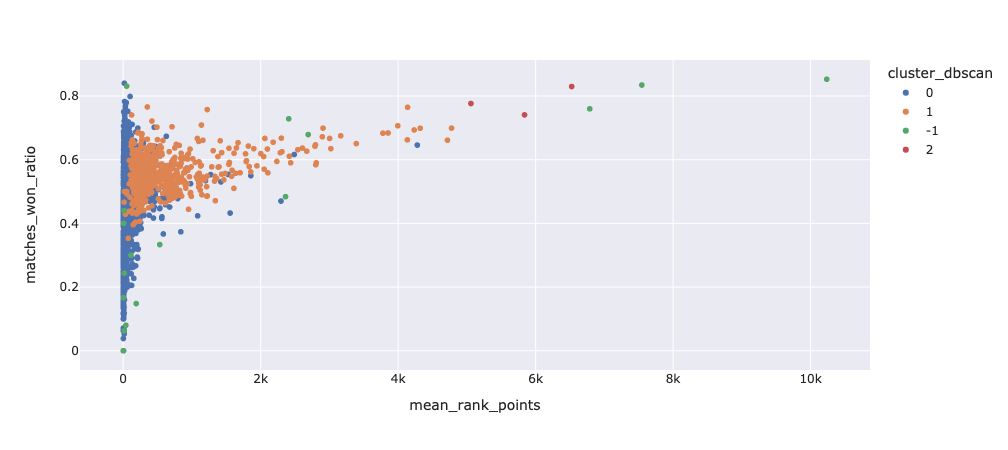
\includegraphics[width=\textwidth]{plots/dbscan/dbscan_results}
\captionof{figure}{Results of DBSCAN}
\label{fig:dbscan_results}
\end{figure}

\subsection{Hierarchical}
As in the DBSCAN we decided to go for a StandardScaler. The dendrogram used to create the cluster was created with a truncate mode $p=9$. The goal was to achieve a more in depth description of the players' profile. While the number of cluster was set to $k=7$ by using the WARD method for the linkage criterion.

\begin{figure}[h]
\centering
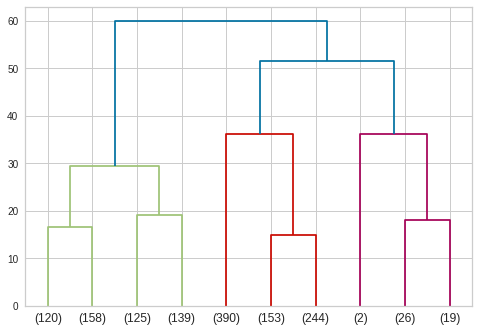
\includegraphics[width=.6\textwidth]{plots/hierarchical/hierarchical_dendrogram}
\captionof{figure}{Results of Hierarchical}
\label{fig:hierarchical_dendrogram}
\end{figure}

\subsubsection{Results interpretation}
The hierarchical clustering subdivided the players in three principal clusters: strong, medium ability and weak players. Strong players were further divided in:
\begin{itemize}
    \item Extremely strong with a very high age and a high number of match played (medium-low last ranking points due to a single player).
    \item Strong on the rise. 
\end{itemize}
Medium ability players were further divided in:
\begin{itemize}
    \item On the rise and young.
    \item In descent and old. 
\end{itemize}
Weak players were further divided in:
\begin{itemize}
    \item In extreme descent and old.
    \item Young promises.
    \item Weak in general.
\end{itemize}
	
\begin{figure}[h]
\centering
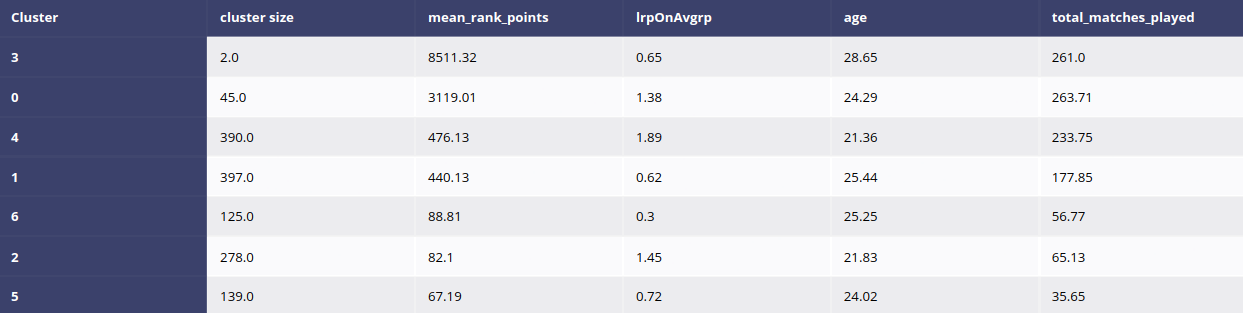
\includegraphics[width=.6\textwidth]{plots/hierarchical/hierarchical_results}
\captionof{figure}{Results of Hierarchical}
\label{fig:hierarchical_results}
\end{figure}

\subsection{Gaussian Mixture}
For the current time being, we tried to exploit the Expectation-Maximization clustering algorithm for Gaussian Mixture Model (GMM) offered by the pyclustering library on the same initially selected features. The algorithm was initialized with a $k=5$ but the output was just $3$ clusters. In the results you can see a behaviour diametrically opposite to that of the DBSCAN, in fact this cluster is focused over the extreme weak players rather than describing with a better accuracy the strong players.  

\begin{itemize}
    \item{ \textbf{Cluster 1} is formed by 1360 players, and it's the biggest one. It's essentially a cluster that described the average profile of a player.}
    \item{ \textbf{Cluster 2} is a small group of 5 weak players that played few matches, but they are improving.}
    \item{\textbf{Cluster 0} is a small group of 11 weak players, but in this case they are younger, and they are not improving so much.}
\end{itemize}

\begin{figure}[h]
\centering
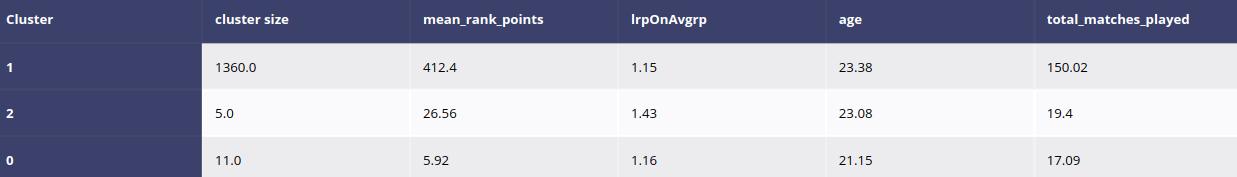
\includegraphics[width=.6\textwidth]{plots/gaussian_mixture//gm_results}
\captionof{figure}{Results of Gaussian Mixture}
\label{fig:gm_results}
\end{figure}

\subsection{Comparison}
Let's compare the different algorithms used and draw conclusions.

\begin{itemize}
    \item{ \textbf{K-means} identifies 4 very even distributions and manages to describe both fairly weak and fairly strong players. And for both it identifies those who are rising and those who are falling.  }
    \item{ \textbf{DBSCAN} is the one that identifies and describes in a better way the players that are excellent at tennis. But it does a poor job in describing all the others, that are just clustered in one huge group.}
    \item{\textbf{Hierarchical} is able to find fairly balanced groups and at the same time maintain a certain flexibility in order to be able to identify the very small group of formidable players. Moreover, it is able to group not only by strong and weak players, but also by intermediate players. In addition, for each group, it is able to identify those on the way up and those on the way down.}
    \item{\textbf{GM}} like DBSCAN but focuses on weak players.
\end{itemize}

In conclusion, the algorithm that manages to describe in the most detailed way the types of players within the dataset is without a doubt the Hierarchy.
